% answers.tex —— 2007 年·普通高等学校招生考试·湖南卷·文科 · 参考答案与详细解析片段
% 由 tools/generate_projects.py 依来源总账自 2007/2007_数学真题_湖南文_试题.md + 2007/2007_数学真题_湖南文_解析正文.md + 2007/2007_数学真题_湖南文_答案要点.md 生成，勿手改（改源 MD 后重跑）


\begin{gktip}
固定候选 PDF 仅含题面，无答案、解析和评分标准，原卷亦未标注分值；以下为非官方编者独立推导，官方答案字段为空。题面文字层只作定位，公式、上下标与三幅图（Q6 正方体、Q7 频率分布直方图、Q18 直二面角）均以 300/400 dpi 原页复核后重绘。
\end{gktip}

\begin{answer}
\gksolhead{1}{}

\textbf{题目}：

不等式 $x^2>x$ 的解集是（　）

（A）$(-\infty,0)$

（B）$(0,1)$

（C）$(1,+\infty)$

（D）$(-\infty,0)\cup(1,+\infty)$

\Needspace{4\baselineskip}
\textbf{解析}

\nopagebreak[4]
\[x^2>x\iff x^2-x>0\iff x(x-1)>0,\]

故 $x<0$ 或 $x>1$，解集为 $(-\infty,0)\cup(1,+\infty)$，选 D。

\gkanswer{答案：D。}

\end{answer}
\begin{answer}
\gksolhead{2}{}

\textbf{题目}：

若 $O$、$E$、$F$ 是不共线的任意三点，则以下各式中成立的是（　）

（A）$\overrightarrow{EF}=\overrightarrow{OF}+\overrightarrow{OE}$

（B）$\overrightarrow{EF}=\overrightarrow{OF}-\overrightarrow{OE}$

（C）$\overrightarrow{EF}=-\overrightarrow{OF}+\overrightarrow{OE}$

（D）$\overrightarrow{EF}=-\overrightarrow{OF}-\overrightarrow{OE}$

\Needspace{4\baselineskip}
\textbf{解析}

\Needspace{5\baselineskip}
由向量减法（终点减起点）：

\nopagebreak[4]
\[\overrightarrow{EF}=\overrightarrow{OF}-\overrightarrow{OE},\]

对应 (B)。其余三式分别等于 $2\overrightarrow{OF}$、$2\overrightarrow{OE}$、$-2\overrightarrow{OF}$ 一类，均不等于 $\overrightarrow{EF}$。

\gkanswer{答案：B。}

\end{answer}
\begin{answer}
\gksolhead{3}{}

\textbf{题目}：

设 $p$：$b^2-4ac>0$（$a\neq0$），$q$：关于 $x$ 的方程 $ax^2+bx+c=0$（$a\neq0$）有实根，则 $p$ 是 $q$ 的（　）

（A）充分不必要条件

（B）必要不充分条件

（C）充分必要条件

（D）既不充分也不必要条件

\Needspace{4\baselineskip}
\textbf{解析}

$p$：$b^2-4ac>0$，即判别式为正，方程有两个不相等的实根，当然有实根，故 $p\Rightarrow q$。

$q$：方程有实根，即 $b^2-4ac\geqslant0$；当 $b^2-4ac=0$ 时 $q$ 成立而 $p$ 不成立，故 $q\not\Rightarrow p$。

所以 $p$ 是 $q$ 的充分不必要条件，选 A。

\gkanswer{答案：A。}

\end{answer}
\begin{answer}
\gksolhead{4}{}

\textbf{题目}：

在等比数列 $\{a_n\}$（$n\in\mathbf N^*$）中，若 $a_1=1$，$a_4=\dfrac18$，则该数列的前 $10$ 项和为（　）

（A）$2-\dfrac1{2^8}$

（B）$2-\dfrac1{2^9}$

（C）$2-\dfrac1{2^{10}}$

（D）$2-\dfrac1{2^{11}}$

\Needspace{4\baselineskip}
\textbf{解析}

\Needspace{5\baselineskip}
设公比为 $q$，由 $a_4=a_1q^3$ 得

\nopagebreak[4]
\[q^3=\frac18\ \Longrightarrow\ q=\frac12 .\]

\Needspace{5\baselineskip}
前 $10$ 项和

\nopagebreak[4]
\[S_{10}=\frac{a_1(1-q^{10})}{1-q}=\frac{1-\left(\frac12\right)^{10}}{\frac12}=2-\frac{1}{2^9},\]

选 B。

（核对：$2-\frac1{512}=\frac{1023}{512}$，而逐项和 $1+\frac12+\cdots+\frac1{512}=\frac{1023}{512}$。）

\gkanswer{答案：B。}

\end{answer}
\begin{answer}
\gksolhead{5}{}

\textbf{题目}：

在 $(1+x)^n$（$n\in\mathbf N^*$）的二项展开式中，若只有 $x^5$ 的系数最大，则 $n=$（　）

（A）$8$

（B）$9$

（C）$10$

（D）$11$

\Needspace{4\baselineskip}
\textbf{解析}

展开式第 $r+1$ 项系数为 $\mathrm C_n^r$。二项式系数先增后减，最大值在中间：

\begin{itemize}
\item $n$ 为偶数时，$r=\frac n2$ 处唯一最大；
\item $n$ 为奇数时，$r=\frac{n-1}{2}$ 与 $r=\frac{n+1}{2}$ 并列最大。
\end{itemize}

题设「只有 $x^5$ 的系数最大」，故 $n$ 为偶数且 $\frac n2=5$，即 $n=10$，选 C。

（校验：$n=10$ 时 $\mathrm C_{10}^5=252$，大于 $\mathrm C_{10}^4=\mathrm C_{10}^6=210$；$n=9$ 时 $\mathrm C_9^4=\mathrm C_9^5=126$ 并列。）

\gkanswer{答案：C。}

\end{answer}
\begin{answer}
\gksolhead{6}{}

\textbf{题目}：

如图，在正四棱柱 $ABCD-A_1B_1C_1D_1$ 中，$E$、$F$ 分别是 $AB_1$、$BC_1$ 的中点，则以下结论中不成立的是（　）
\nopagebreak[4]
\begin{center}% 2007 年湖南卷文科第 6 题：正四棱柱 ABCD-A_1B_1C_1D_1，E、F 分别为 AB_1、BC_1 的中点。
% 来源 PDF：普通高考/2007/2007湖南文.pdf，SHA256 8e889ae321ffa864b24c505b40e7e96956b301487f5a106264b7fcd9f943e068
% 原页：第 1 页（A3 三栏）第 1 栏下部，印刷页 381，图在题干下方。
% 重绘依据：斜投影正方体，A 左下、B 右下、C 右后、D 左后，上底同名加下标 1；
%   可见棱与上底对角线 A_1C_1 实线，被遮棱 D-D_1、C-D、D-A 与上底对角线 B_1D_1 虚线；
%   E 在 AB_1 上、F 在 BC_1 上，均取中点并画小黑点；标注位置按原图。
\begin{tikzpicture}[scale=1.05, semithick,
  every node/.style={inner sep=1.5pt}]
  \coordinate (A)  at (0,0);
  \coordinate (B)  at (2.4,0);
  \coordinate (D)  at (0.9,0.6);
  \coordinate (C)  at (3.3,0.6);
  \coordinate (A1) at (0,2.4);
  \coordinate (B1) at (2.4,2.4);
  \coordinate (D1) at (0.9,3.0);
  \coordinate (C1) at (3.3,3.0);
  % 被遮棱
  \draw[dashed] (D) -- (D1);
  \draw[dashed] (C) -- (D);
  \draw[dashed] (D) -- (A);
  % 可见棱
  \draw (A) -- (B) -- (C) -- (C1) -- (D1) -- (A1) -- cycle;
  \draw (A) -- (A1);
  \draw (B) -- (B1);
  \draw (C) -- (C1);
  \draw (B1) -- (C1);
  \draw (A1) -- (B1);
  % 上底对角线
  \draw (A1) -- (C1);
  \draw[dashed] (B1) -- (D1);
  % 两条侧面对角线（E、F 所在）
  \draw (A) -- (B1);
  \draw (B) -- (C1);
  % E、F
  \coordinate (E) at ($(A)!0.5!(B1)$);
  \coordinate (F) at ($(B)!0.5!(C1)$);
  \fill (E) circle (1.4pt);
  \fill (F) circle (1.4pt);
  \node[anchor=east]  at ([xshift=-2pt]E) {$E$};
  \node[anchor=west]  at ([xshift=2pt]F) {$F$};
  % 顶点标注
  \node[anchor=north east] at (A)  {$A$};
  \node[anchor=north west] at (B)  {$B$};
  \node[anchor=west]       at (C)  {$C$};
  \node[anchor=east]       at (D)  {$D$};
  \node[anchor=south east] at (A1) {$A_1$};
  \node[anchor=south west] at (B1) {$B_1$};
  \node[anchor=south west] at (C1) {$C_1$};
  \node[anchor=south east] at (D1) {$D_1$};
\end{tikzpicture}
\end{center}
\nopagebreak[4]
（A）$EF$ 与 $BB_1$ 垂直

（B）$EF$ 与 $BD$ 垂直

（C）$EF$ 与 $CD$ 异面

（D）$EF$ 与 $A_1C_1$ 异面

\Needspace{4\baselineskip}
\textbf{解析}

\Needspace{5\baselineskip}
设棱长为 $1$，以 $A$ 为原点、$AB$、$AD$、$AA_1$ 为坐标轴：

\nopagebreak[4]
\[A(0,0,0),\ B(1,0,0),\ C(1,1,0),\ D(0,1,0),\]
\nopagebreak[4]
\[A_1(0,0,1),\ B_1(1,0,1),\ C_1(1,1,1),\ D_1(0,1,1).\]

\Needspace{5\baselineskip}
$E$ 为 $AB_1$ 中点，$F$ 为 $BC_1$ 中点，故

\nopagebreak[4]
\[E\left(\frac12,0,\frac12\right),\qquad F\left(1,\frac12,\frac12\right),\qquad \overrightarrow{EF}=\left(\frac12,\frac12,0\right).\]

逐项判断：

(A) $\overrightarrow{BB_1}=(0,0,1)$，$\overrightarrow{EF}\cdot\overrightarrow{BB_1}=0$，垂直，成立。

(B) $\overrightarrow{BD}=(-1,1,0)$，$\overrightarrow{EF}\cdot\overrightarrow{BD}=-\frac12+\frac12=0$，垂直，成立。

(C) $CD$ 在平面 $z=0$ 内、方向沿 $x$ 轴负向；$EF$ 在平面 $z=\frac12$ 内、方向 $(1,1,0)$。两直线方向不平行，且无公共点，故异面，成立。

(D) $\overrightarrow{A_1C_1}=(1,1,0)=2\overrightarrow{EF}$，两直线平行，不是异面，不成立。

故选 D。

\gkanswer{答案：D。}

\end{answer}
\begin{answer}
\gksolhead{7}{}

\textbf{题目}：

根据某水文观测点的历史统计数据，得到某条河流水位的频率分布直方图（如图），从图中可以看出，该水文观测点平均至少一百年才遇到一次的洪水的最低水位是（　）
\nopagebreak[4]
\begin{center}% 2007 年湖南卷文科第 7 题：河流水位的频率分布直方图。
% 来源 PDF：普通高考/2007/2007湖南文.pdf，SHA256 8e889ae321ffa864b24c505b40e7e96956b301487f5a106264b7fcd9f943e068
% 原页：第 1 页（A3 三栏）第 2 栏上部，印刷页 381，图在题干下方。
% 重绘依据：横轴水位 30–51 米、组距 1 米；纵轴为频率/组距，标出 0.5%、1%、2% 三条虚线。
%   逐柱高度按原图柱顶量取（以 1% 线为标尺），再按「各组频率之和为 100%」归一：
%   30–31 为 2.6%、31–32 为 3.1%、32–33 为 3.4%，其后渐升，39–40 达峰 8.0%，
%   43–47 有起伏；尾三组按原图标注取 48–49 为 2.0%、49–50 为 1.0%、50–51 为 0.5%。
%   原图只在两端标出 30–33 与 48–51，此处照录。
\begin{tikzpicture}[scale=0.60, semithick, every node/.style={inner sep=1.5pt}]
  % 坐标轴
  \draw[->] (29.7,0) -- (51.9,0) node[anchor=west] {水位（米）};
  \draw[->] (30,0) -- (30,7.6);
  \node[align=center, anchor=south] at (30,7.65) {频率\\[-1pt]组距};
  % 断裂记号
  \draw (29.85,0) -- (29.95,0.12) -- (30.05,-0.02);
  % 三条水平虚线
  \draw[dashed] (30,0.5) -- (51.4,0.5);
  \node[anchor=east] at (29.92,0.5) {$0.5\%$};
  \draw[dashed] (30,1) -- (51.4,1);
  \node[anchor=east] at (29.92,1) {$1\%$};
  \draw[dashed] (30,2) -- (51.4,2);
  \node[anchor=east] at (29.92,2) {$2\%$};
  % 各柱
  \foreach \x/\h in {
    30/2.6, 31/3.1, 32/3.4, 33/3.9, 34/4.5, 35/5.1, 36/5.8,
    37/6.2, 38/6.6, 39/8.0, 40/7.5, 41/6.9, 42/6.3, 43/5.2,
    44/5.8, 45/5.4, 46/5.8, 47/4.8, 48/2.0, 49/1.0, 50/0.5} {
    \draw (\x,\h) rectangle (\x+1,0);
  }
  % 横轴刻度标签（照原图只标两端）
  \foreach \x in {30,31,32,33,48,49,50,51} {
    \node[anchor=north] at (\x,-0.04) {\x};
  }
\end{tikzpicture}
\end{center}
\nopagebreak[4]
（A）$48$ 米

（B）$49$ 米

（C）$50$ 米

（D）$51$ 米

\Needspace{4\baselineskip}
\textbf{解析}

「平均至少一百年才遇到一次」即重现期 $T\geqslant100$，对应年超越概率不超过 $1\%$。

\Needspace{5\baselineskip}
读直方图：$48$–$49$ 米一组为 $2\%$，$49$–$50$ 米一组为 $1\%$，$50$–$51$ 米一组为 $0.5\%$。对水位阈值 $L$，年超越概率是「水位不低于 $L$」的各组频率之和：

\nopagebreak[4]
\[P(X\geqslant49)=1\%+0.5\%=1.5\%>1\%,\]

\nopagebreak[4]
\[P(X\geqslant50)=0.5\%\leqslant1\% .\]

故 $49$ 米约 $67$ 年一遇，不满足；$50$ 米约 $200$ 年一遇，满足。最低水位为 $50$ 米，选 C。

\gkanswer{答案：C。}

\end{answer}
\begin{answer}
\gksolhead{8}{}

\textbf{题目}：

函数 $f(x)=\begin{cases}4x-4,&x\leqslant1,\\ x^2-4x+3,&x>1,\end{cases}$ 的图象和函数 $g(x)=\log_2 x$ 的图象的交点个数是（　）

（A）$1$

（B）$2$

（C）$3$

（D）$4$

\Needspace{4\baselineskip}
\textbf{解析}

分段讨论。

$x\leqslant1$：$f(x)=4x-4$，$g(x)=\log_2x$。

\begin{itemize}
\item $x=1$ 时 $f(1)=0=g(1)$，是一个交点。
\item $0<x<1$ 时，$f$ 从 $-4$ 单调增到 $0$，$g$ 从 $-\infty$ 单调增到 $0$。取 $x=0.1$：$f=-3.6$，$g\approx-3.32$，$f<g$；取 $x\to0^+$：$f\to-4$，$g\to-\infty$，$f>g$。故在 $(0,0.1)$ 内有一个交点。
\end{itemize}

$x>1$：$f(x)=x^2-4x+3$。

\begin{itemize}
\item $1<x<3$ 时 $f(x)<0<g(x)$，无交点；
\item $x=3$ 时 $f=0<g\approx1.585$；$x=4$ 时 $f=3>g=2$，故在 $(3,4)$ 内有一个交点；
\item 在 $(3,+\infty)$ 上 $f$ 的增长速度最终快于 $g$，且 $h(x)=x^2-4x+3-\log_2x$ 在 $x>2$ 时先减后增、只有一个零点，故该区间只有一个交点。
\end{itemize}

共 $3$ 个交点，选 C。

\gkanswer{答案：C。}

\end{answer}
\begin{answer}
\gksolhead{9}{}

\textbf{题目}：

设 $F_1$、$F_2$ 分别是椭圆 $\dfrac{x^2}{a^2}+\dfrac{y^2}{b^2}=1$（$a>b>1$）的左、右焦点，$P$ 是其右准线上纵坐标为 $\sqrt3c$（$c$ 为半焦距）的点，且 $|F_1F_2|=|F_2P|$，则椭圆的离心率是（　）

（A）$\dfrac{\sqrt3-1}{2}$

（B）$\dfrac12$

（C）$\dfrac{\sqrt5-1}{2}$

（D）$\dfrac{\sqrt2}{2}$

\Needspace{4\baselineskip}
\textbf{解析}

\Needspace{5\baselineskip}
椭圆右准线为 $x=\frac{a^2}{c}$，故 $P\left(\frac{a^2}{c},\sqrt3c\right)$。又 $F_2(c,0)$，

\nopagebreak[4]
\[|F_2P|^2=\left(\frac{a^2}{c}-c\right)^2+(\sqrt3c)^2=\left(\frac{a^2-c^2}{c}\right)^2+3c^2=\frac{b^4}{c^2}+3c^2 .\]

\Needspace{5\baselineskip}
由 $|F_1F_2|=2c$ 及题设：

\nopagebreak[4]
\[4c^2=\frac{b^4}{c^2}+3c^2\ \Longrightarrow\ c^2=\frac{b^4}{c^2}\ \Longrightarrow\ c^4=b^4\ \Longrightarrow\ b=c .\]

于是 $a^2=b^2+c^2=2c^2$，$e=\frac ca=\frac{1}{\sqrt2}=\frac{\sqrt2}{2}$，选 D。

\gkanswer{答案：D。}

\end{answer}
\begin{answer}
\gksolhead{10}{}

\textbf{题目}：

设集合 $M=\{1,2,3,4,5,6\}$，$S_1$、$S_2$、…、$S_k$ 都是 $M$ 的含两个元素的子集，且满足：对任意的 $S_i=\{a_i,b_i\}$，$S_j=\{a_j,b_j\}$（$i\neq j$，$i$、$j\in\{1,2,3,\cdots,k\}$），都有 $\min\left\{\dfrac{a_i}{b_i},\dfrac{b_i}{a_i}\right\}\neq\min\left\{\dfrac{a_j}{b_j},\dfrac{b_j}{a_j}\right\}$（$\min\{x,y\}$ 表示两个数 $x$、$y$ 中的较小者）．则 $k$ 的最大值是（　）

（A）$10$

（B）$11$

（C）$12$

（D）$13$

\Needspace{4\baselineskip}
\textbf{解析}

\Needspace{5\baselineskip}
对二元子集 $\{a,b\}$（$a<b$），

\nopagebreak[4]
\[\min\left\{\frac ab,\frac ba\right\}=\frac ab .\]

列出 $M=\{1,2,3,4,5,6\}$ 的全部 $15$ 个二元子集及其比值：

\begin{center}
\begin{tabular}{ll}
\toprule
比值 & 子集 \\
\midrule
$\frac16$ & $\{1,6\}$ \\
$\frac15$ & $\{1,5\}$ \\
$\frac14$ & $\{1,4\}$ \\
$\frac13$ & $\{1,3\},\{2,6\}$ \\
$\frac25$ & $\{2,5\}$ \\
$\frac12$ & $\{1,2\},\{2,4\},\{3,6\}$ \\
$\frac35$ & $\{3,5\}$ \\
$\frac23$ & $\{2,3\},\{4,6\}$ \\
$\frac34$ & $\{3,4\}$ \\
$\frac45$ & $\{4,5\}$ \\
$\frac56$ & $\{5,6\}$ \\
\bottomrule
\end{tabular}
\end{center}

不同比值共 $11$ 个。题设要求任意两个子集对应的 $\min$ 值互不相等，故同一比值的多个子集至多取一个。每个不同比值各取一个代表，即可得到 $11$ 个子集，故 $k_{\max}=11$，选 B。

\gkanswer{答案：B。}

\end{answer}
\begin{answer}
\gksolhead{11}{}

\textbf{题目}：

圆心为 $(1,1)$ 且与直线 $x+y=4$ 相切的圆的方程是\gkblank{}．

\Needspace{4\baselineskip}
\textbf{解析}

\Needspace{5\baselineskip}
圆心 $(1,1)$ 到直线 $x+y-4=0$ 的距离即半径：

\nopagebreak[4]
\[r=\frac{|1+1-4|}{\sqrt{1^2+1^2}}=\frac{2}{\sqrt2}=\sqrt2 .\]

\Needspace{5\baselineskip}
故圆的方程为

\nopagebreak[4]
\[(x-1)^2+(y-1)^2=2 .\]

\gkanswer{答案：$(x-1)^2+(y-1)^2=2$。}

\end{answer}
\begin{answer}
\gksolhead{12}{}

\textbf{题目}：

在 $\triangle ABC$ 中，角 $A$、$B$、$C$ 所对的边分别为 $a$、$b$、$c$，若 $a=1$，$c=\sqrt3$，$C=\dfrac{\pi}{3}$，则 $A=$\gkblank{}．

\Needspace{4\baselineskip}
\textbf{解析}

\Needspace{5\baselineskip}
由正弦定理

\nopagebreak[4]
\[\frac{a}{\sin A}=\frac{c}{\sin C},\]

\Needspace{5\baselineskip}
得

\nopagebreak[4]
\[\sin A=\frac{a\sin C}{c}=\frac{1\cdot\frac{\sqrt3}{2}}{\sqrt3}=\frac12 .\]

\Needspace{5\baselineskip}
故 $A=\frac{\pi}{6}$ 或 $\frac{5\pi}{6}$。又 $a=1<c=\sqrt3$，故 $A<C=\frac{\pi}{3}$，只能取

\nopagebreak[4]
\[A=\frac{\pi}{6}.\]

\gkanswer{答案：$\frac{\pi}{6}$。}

\end{answer}
\begin{answer}
\gksolhead{13}{}

\textbf{题目}：

若 $a>0$，$a^{\frac23}=\dfrac49$，则 $\log_{\frac23}a=$\gkblank{}．

\Needspace{4\baselineskip}
\textbf{解析}

\Needspace{5\baselineskip}
由 $a^{\frac23}=\frac49$ 得

\nopagebreak[4]
\[a=\left(\frac49\right)^{\frac32}=\left(\frac23\right)^3=\frac{8}{27}.\]

\Needspace{5\baselineskip}
于是

\nopagebreak[4]
\[\log_{\frac23}a=\log_{\frac23}\left(\frac23\right)^3=3 .\]

\gkanswer{答案：$3$。}

\end{answer}
\begin{answer}
\gksolhead{14}{}

\textbf{题目}：

设集合 $A=\left\{(x,y)\mid y\geqslant|x-2|,\ x\geqslant0\right\}$，$B=\left\{(x,y)\mid y\leqslant-x+b\right\}$，$A\cap B\neq\varnothing$．

（1）$b$ 的取值范围是\gkblank{}；

（2）若 $(x,y)\in A\cap B$，且 $x+2y$ 的最大值为 $9$，则 $b$ 的值是\gkblank{}．

\Needspace{4\baselineskip}
\textbf{解析}

\Needspace{5\baselineskip}
（1）$A$ 为折线 $y=|x-2|$ 上方的区域（$x\geqslant0$），顶点为 $(2,0)$。直线 $l:y=-x+b$ 的纵截距为 $b$，要与 $A$ 相交，至少要经过顶点 $(2,0)$：

\nopagebreak[4]
\[0=-2+b\ \Longrightarrow\ b=2,\]

故 $b\geqslant2$。

\Needspace{5\baselineskip}
（2）在 $A\cap B$ 上，对每个固定的 $x$，取 $y$ 的最大可能值 $y=b-x$（需满足 $b-x\geqslant|x-2|$），则

\nopagebreak[4]
\[x+2y\leqslant x+2(b-x)=2b-x .\]

\Needspace{5\baselineskip}
当 $x\geqslant0$ 时，$2b-x\leqslant2b$，等号在 $x=0$ 处取得；此时 $y=b$，且 $b\geqslant2$ 保证 $b\geqslant|0-2|=2$，点 $(0,b)$ 确在 $A\cap B$ 内。故最大值为 $2b$。由

\nopagebreak[4]
\[2b=9\ \Longrightarrow\ b=\frac92 .\]

\gkanswer{答案：（1）$b\geqslant2$；（2）$\frac92$。}

\end{answer}
\begin{answer}
\gksolhead{15}{}

\textbf{题目}：

棱长为 $1$ 的正方体 $ABCD-A_1B_1C_1D_1$ 的 $8$ 个顶点都在球 $O$ 的表面上，则球 $O$ 的表面积是\gkblank{}；设 $E$、$F$ 分别是该正方体的棱 $AA_1$、$DD_1$ 的中点，则直线 $EF$ 被球 $O$ 截得的线段长为\gkblank{}．

\Needspace{4\baselineskip}
\textbf{解析}

\Needspace{5\baselineskip}
正方体的体对角线为外接球直径：

\nopagebreak[4]
\[2R=\sqrt{1^2+1^2+1^2}=\sqrt3\ \Longrightarrow\ R=\frac{\sqrt3}{2}.\]

\Needspace{5\baselineskip}
球表面积

\nopagebreak[4]
\[S=4\pi R^2=4\pi\cdot\frac34=3\pi .\]

\Needspace{5\baselineskip}
取坐标 $A(0,0,0)$、$B(1,0,0)$、$D(0,1,0)$、$A_1(0,0,1)$、$D_1(0,1,1)$。则

\nopagebreak[4]
\[E\left(0,0,\frac12\right),\quad F\left(0,1,\frac12\right),\quad O\left(\frac12,\frac12,\frac12\right).\]

\Needspace{5\baselineskip}
直线 $EF$ 为 $x=0,\ z=\frac12$，$O$ 到它的垂足为 $\left(0,\frac12,\frac12\right)$，距离 $d=\frac12$。故截得弦长

\nopagebreak[4]
\[2\sqrt{R^2-d^2}=2\sqrt{\frac34-\frac14}=\sqrt2 .\]

\gkanswer{答案：$3\pi$；$\sqrt2$。}

\end{answer}
\begin{answer}
\gksolhead{16}{}

\textbf{题目}：

已知函数 $f(x)=1-2\sin^2\left(x+\dfrac{\pi}{8}\right)+2\sin\left(x+\dfrac{\pi}{8}\right)\cos\left(x+\dfrac{\pi}{8}\right)$．求：

（1）函数 $f(x)$ 的最小正周期；

（2）函数 $f(x)$ 的单调增区间．

\Needspace{4\baselineskip}
\textbf{解析}

\Needspace{5\baselineskip}
令 $t=x+\frac{\pi}{8}$。则

\nopagebreak[4]
\[1-2\sin^2t=\cos2t,\qquad 2\sin t\cos t=\sin2t,\]

\Needspace{5\baselineskip}
故

\nopagebreak[4]
\[
\begin{aligned}
f(x)&=\cos2t+\sin2t=\sqrt2\sin\left(2t+\frac{\pi}{4}\right)\\
&=\sqrt2\sin\left(2x+\frac{\pi}{4}+\frac{\pi}{4}\right)
=\sqrt2\sin\left(2x+\frac{\pi}{2}\right)=\sqrt2\cos2x .
\end{aligned}
\]

（1）最小正周期 $T=\frac{2\pi}{2}=\pi$。

\Needspace{5\baselineskip}
（2）$f'(x)=-2\sqrt2\sin2x$。由 $f'(x)>0$ 得 $\sin2x<0$，即

\nopagebreak[4]
\[2x\in(\pi+2k\pi,\ 2\pi+2k\pi),\]

\Needspace{5\baselineskip}
故

\nopagebreak[4]
\[x\in\left(\frac{\pi}{2}+k\pi,\ \pi+k\pi\right),\quad k\in\mathbf Z .\]

单调增区间为 $\left[\frac{\pi}{2}+k\pi,\ \pi+k\pi\right]$（$k\in\mathbf Z$）。

\gkanswer{答案：（1）$\pi$；（2）$\left[\frac{\pi}{2}+k\pi,\ \pi+k\pi\right]$（$k\in\mathbf Z$）。}

\end{answer}
\begin{answer}
\gksolhead{17}{}

\textbf{题目}：

某地区为下岗人员免费提供财会和计算机培训，以提高下岗人员的再就业能力．每名下岗人员可以选择参加一项培训、参加两项培训或不参加培训，已知参加过财会培训的有 $60\%$，参加过计算机培训的有 $75\%$．假设每个人对培训项目的选择是相互独立的，且各人的选择相互之间没有影响．

（1）任选 $1$ 名下岗人员，求该人参加过培训的概率；

（2）任选 $3$ 名下岗人员，求这 $3$ 人中至少有 $2$ 人参加过培训的概率．

\Needspace{4\baselineskip}
\textbf{解析}

设 $A$＝参加过财会培训，$B$＝参加过计算机培训，$P(A)=0.6$、$P(B)=0.75$，且 $A$、$B$ 独立。

\Needspace{5\baselineskip}
（1）至少参加一项：

\nopagebreak[4]
\[P(A\cup B)=P(A)+P(B)-P(A)P(B)=0.6+0.75-0.6\times0.75=1.35-0.45=0.9 .\]

\Needspace{5\baselineskip}
（2）任选 $3$ 人，设参加过培训的人数为 $X$，每人参加的概率为 $0.9$ 且相互独立，故 $X\sim B(3,0.9)$。

\nopagebreak[4]
\[
\begin{aligned}
P(X\geqslant2)&=P(X=2)+P(X=3)\\
&=\mathrm C_3^2(0.9)^2(0.1)+(0.9)^3
=3\times0.081+0.729=0.243+0.729=0.972 .
\end{aligned}
\]

\gkanswer{答案：（1）$0.9$；（2）$0.972$。}

\end{answer}
\begin{answer}
\gksolhead{18}{}

\textbf{题目}：

如图，已知直二面角 $\alpha-PQ-\beta$，$A\in PQ$，$B\in\alpha$，$C\in\beta$，$CA=CB$，$\angle BAP=45^\circ$，直线 $CA$ 和平面 $\alpha$ 所成的角为 $30^\circ$．
\nopagebreak[4]
\begin{center}% 2007 年湖南卷文科第 18 题：直二面角 α-PQ-β，A∈PQ，B∈α，C∈β。
% 来源 PDF：普通高考/2007/2007湖南文.pdf，SHA256 8e889ae321ffa864b24c505b40e7e96956b301487f5a106264b7fcd9f943e068
% 原页：第 2 页（A3 三栏）第 1 栏上部，印刷页 382，图在题干下方。
% 重绘依据：β 画成上半平面（竖直矩形），α 画成下半平面（平行四边形），交线 PQ 水平；
%   P 在左端、A 在 P 右侧、Q 在 A 右侧；C 在 β 内、B 在 α 内；
%   线段 CA、CB、AB 实线，平面轮廓与交线细实线，标注按原图。
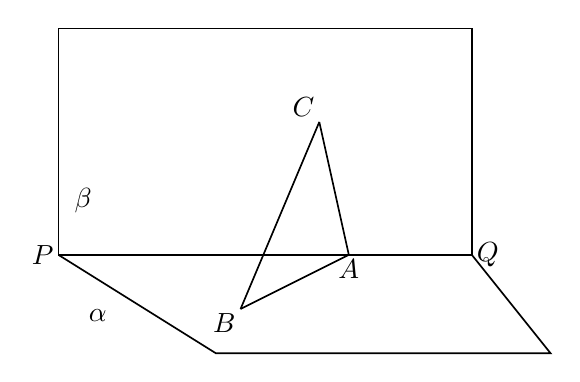
\begin{tikzpicture}[scale=1.25, semithick, every node/.style={inner sep=1.5pt}]
  % 平面 β（上）与 α（下）
  \draw (-2.6,0) -- (1.6,0) -- (1.6,2.3) -- (-2.6,2.3) -- cycle;
  \draw (-2.6,0) -- (-1.0,-1.0) -- (2.4,-1.0) -- (1.6,0);
  % 交线 PQ
  \draw (-2.6,0) -- (1.6,0);
  % 点
  \coordinate (P) at (-2.6,0);
  \coordinate (A) at (0.35,0);
  \coordinate (Q) at (1.6,0);
  \coordinate (C) at (0.05,1.35);
  \coordinate (B) at (-0.75,-0.55);
  % 关键线段
  \draw (C) -- (A);
  \draw (C) -- (B);
  \draw (A) -- (B);
  % 标注
  \node[anchor=east]  at (P) {$P$};
  \node[anchor=north] at (A) {$A$};
  \node[anchor=west]  at (Q) {$Q$};
  \node[anchor=south east] at (C) {$C$};
  \node[anchor=north east] at (B) {$B$};
  \node at (-2.35,0.55) {$\beta$};
  \node at (-2.2,-0.62) {$\alpha$};
\end{tikzpicture}
\end{center}
\nopagebreak[4]
（1）证明：$BC\perp PQ$；

（2）求二面角 $B-AC-P$ 的大小．

\Needspace{4\baselineskip}
\textbf{解析}

（1）直二面角 $\alpha-PQ-\beta$ 的平面角为 $90^\circ$，故平面 $\alpha\perp$ 平面 $\beta$，交线为 $PQ$。

以 $PQ$ 为 $x$ 轴、$\alpha$ 为 $xy$ 平面、$\beta$ 为 $xz$ 平面建立坐标系，设 $A(0,0,0)$，$AP$ 沿 $-x$ 方向。由 $B\in\alpha$，设 $B(-s,s,0)$（$\angle BAP=45^\circ$）；由 $C\in\beta$，设 $C(u,0,w)$。

\Needspace{5\baselineskip}
$CA=CB$ 给出

\nopagebreak[4]
\[|C|^2=|B-C|^2\ \Longrightarrow\ |B|^2=2\overrightarrow{OB}\cdot\overrightarrow{OC},\]

\Needspace{5\baselineskip}
即 $2s^2=2(-su)$，故 $u=-s$。又直线 $CA$ 与平面 $\alpha$ 所成角为 $30^\circ$：

\nopagebreak[4]
\[\frac{|w|}{\sqrt{u^2+w^2}}=\frac12\ \Longrightarrow\ 4w^2=u^2+w^2\ \Longrightarrow\ w^2=\frac{u^2}{3},\]

\Needspace{5\baselineskip}
取 $w=\frac{s}{\sqrt3}$。于是

\nopagebreak[4]
\[C\left(-s,0,\frac{s}{\sqrt3}\right),\qquad \overrightarrow{BC}=\left(0,-s,\frac{s}{\sqrt3}\right).\]

而 $PQ$ 的方向向量为 $(1,0,0)$，$\overrightarrow{BC}\cdot(1,0,0)=0$，故 $BC\perp PQ$。

\Needspace{5\baselineskip}
（2）平面 $ACP$ 就是 $\beta$（$xz$ 平面），取法向量 $\mathbf n_1=(0,1,0)$。平面 $ACB$ 的法向量

\nopagebreak[4]
\[\mathbf n_2=\overrightarrow{AC}\times\overrightarrow{AB}
=\left(-s,0,\frac{s}{\sqrt3}\right)\times(-s,s,0)
=\left(-\frac{s^2}{\sqrt3},-\frac{s^2}{\sqrt3},-s^2\right),\]

\Needspace{5\baselineskip}
取 $\mathbf n_2=\left(-\frac1{\sqrt3},-\frac1{\sqrt3},-1\right)$。则

\nopagebreak[4]
\[\cos\theta=\frac{|\mathbf n_1\cdot\mathbf n_2|}{|\mathbf n_1||\mathbf n_2|}
=\frac{\frac1{\sqrt3}}{\sqrt{\frac13+\frac13+1}}
=\frac{1}{\sqrt5}.\]

\Needspace{5\baselineskip}
故

\nopagebreak[4]
\[\theta=\arccos\frac{\sqrt5}{5}=\arctan2\approx63.4^\circ .\]

（方向核对：在垂直于 $AC$ 的截面内，指向 $B$ 与指向 $P$ 的两条射线夹角余弦为正，取锐角。）

\gkanswer{答案：（1）证明见解析；（2）$\arccos\frac{\sqrt5}{5}$（即 $\arctan2$，约 $63.4^\circ$）。}

\end{answer}
\begin{answer}
\gksolhead{19}{}

\textbf{题目}：

已知双曲线 $x^2-y^2=2$ 的右焦点为 $F$，过点 $F$ 的动直线与双曲线相交于 $A$、$B$ 两点，点 $C$ 的坐标是 $(1,0)$．

（1）证明：$\overrightarrow{CA}\cdot\overrightarrow{CB}$ 为常数；

（2）若动点 $M$ 满足 $\overrightarrow{CM}=\overrightarrow{CA}+\overrightarrow{CB}+\overrightarrow{CO}$（其中 $O$ 为坐标原点），求点 $M$ 的轨迹方程．

\Needspace{4\baselineskip}
\textbf{解析}

双曲线 $x^2-y^2=2$ 即 $\frac{x^2}{2}-\frac{y^2}{2}=1$，$c=\sqrt{2+2}=2$，右焦点 $F(2,0)$。

\Needspace{5\baselineskip}
（1）设过 $F$ 的直线为 $x=my+2$，代入双曲线：

\nopagebreak[4]
\[(my+2)^2-y^2=2\ \Longrightarrow\ (m^2-1)y^2+4my+2=0 .\]

\Needspace{5\baselineskip}
设 $A(x_1,y_1)$、$B(x_2,y_2)$，则

\nopagebreak[4]
\[y_1+y_2=-\frac{4m}{m^2-1},\qquad y_1y_2=\frac{2}{m^2-1}.\]

\Needspace{5\baselineskip}
由 $x_i=my_i+2$ 得 $x_i-1=my_i+1$，故

\nopagebreak[4]
\[\overrightarrow{CA}\cdot\overrightarrow{CB}=(my_1+1)(my_2+1)+y_1y_2
=(m^2+1)y_1y_2+m(y_1+y_2)+1 .\]

\Needspace{5\baselineskip}
代入：

\nopagebreak[4]
\[=(m^2+1)\cdot\frac{2}{m^2-1}+m\cdot\left(-\frac{4m}{m^2-1}\right)+1
=\frac{2m^2+2-4m^2}{m^2-1}+1=-2+1=-1 .\]

当直线为 $x=2$（$m=0$）时，$A(2,\sqrt2)$、$B(2,-\sqrt2)$，$\overrightarrow{CA}\cdot\overrightarrow{CB}=1-2=-1$，同样成立。故 $\overrightarrow{CA}\cdot\overrightarrow{CB}=-1$ 为常数。

\Needspace{5\baselineskip}
（2）由

\nopagebreak[4]
\[\overrightarrow{CM}=\overrightarrow{CA}+\overrightarrow{CB}+\overrightarrow{CO}\]

\Needspace{5\baselineskip}
及 $C(1,0)$、$O(0,0)$，得

\nopagebreak[4]
\[M=C+\overrightarrow{CM}=(1,0)+(x_1-1,y_1)+(x_2-1,y_2)+(-1,0)
=(x_1+x_2-2,\ y_1+y_2).\]

\Needspace{5\baselineskip}
由韦达定理，

\nopagebreak[4]
\[x_1+x_2=m(y_1+y_2)+4=-\frac{4m^2}{m^2-1}+4=-\frac{4}{m^2-1},\]

\Needspace{5\baselineskip}
故

\nopagebreak[4]
\[x_M=-\frac{4}{m^2-1}-2=-\frac{2(m^2+1)}{m^2-1},\qquad y_M=-\frac{4m}{m^2-1}.\]

\Needspace{5\baselineskip}
于是

\nopagebreak[4]
\[x_M+2=-\frac{4}{m^2-1},\qquad x_M-2=-\frac{4m^2}{m^2-1},\]

\Needspace{5\baselineskip}
从而

\nopagebreak[4]
\[x_M^2-4-y_M^2=(x_M+2)(x_M-2)-y_M^2
=\frac{16m^2}{(m^2-1)^2}-\frac{16m^2}{(m^2-1)^2}=0 .\]

\Needspace{5\baselineskip}
当直线为 $y=0$ 时，$A(\sqrt2,0)$、$B(-\sqrt2,0)$，$M=(-2,0)$，也满足。故轨迹方程为

\nopagebreak[4]
\[x^2-y^2=4 .\]

\gkanswer{答案：（1）$\overrightarrow{CA}\cdot\overrightarrow{CB}=-1$；（2）$x^2-y^2=4$。}

\end{answer}
\begin{answer}
\gksolhead{20}{}

\textbf{题目}：

设 $S_n$ 是数列 $\{a_n\}$（$n\in\mathbf N^*$）的前 $n$ 项和，$a_1=a$，且 $S_n^2=3n^2a_n+S_{n-1}^2$，$a_n\neq0$，$n=2,3,4,\cdots$．

（1）证明：数列 $\{a_{n+2}-a_n\}$（$n\geqslant2$）是常数数列；

（2）试找出一个奇数 $a$，使以 $18$ 为首项，$7$ 为公比的等比数列 $\{b_n\}$（$n\in\mathbf N^*$）中的所有项都是数列 $\{a_n\}$ 中的项，并指出 $b_n$ 是数列 $\{a_n\}$ 中的第几项．

\Needspace{4\baselineskip}
\textbf{解析}

\Needspace{5\baselineskip}
（1）由 $S_n^2-S_{n-1}^2=a_n(S_n+S_{n-1})$ 及题设 $S_n^2=3n^2a_n+S_{n-1}^2$，得

\nopagebreak[4]
\[a_n(S_n+S_{n-1})=3n^2a_n .\]

\Needspace{5\baselineskip}
因 $a_n\neq0$（$n\geqslant2$），故

\nopagebreak[4]
\[S_n+S_{n-1}=3n^2\quad(n\geqslant2).\]

\Needspace{5\baselineskip}
把 $n$ 换成 $n+1$：

\nopagebreak[4]
\[S_{n+1}+S_n=3(n+1)^2 .\]

\Needspace{5\baselineskip}
两式相减：

\nopagebreak[4]
\[a_{n+1}+a_n=3\left[(n+1)^2-n^2\right]=6n+3 .\]

\Needspace{5\baselineskip}
再对 $n+1$ 写一次并相减：

\nopagebreak[4]
\[(a_{n+2}+a_{n+1})-(a_{n+1}+a_n)=6(n+1)+3-(6n+3)=6,\]

\Needspace{5\baselineskip}
即

\nopagebreak[4]
\[a_{n+2}-a_n=6\quad(n\geqslant2),\]

为常数。

（2）由 $S_2+S_1=12$ 得 $(a_1+a_2)+a_1=12$，即 $a_2=12-2a$。

\Needspace{5\baselineskip}
对 $n\geqslant2$，由 $a_{n+1}=-a_n+6n+3$ 及 $a_2=12-2a$ 解得

\nopagebreak[4]
\[a_n=3n+(6-2a)(-1)^n .\]

\Needspace{5\baselineskip}
取 $a=3$（奇数），则 $6-2a=0$，故 $a_n=3n$（$n\geqslant2$）；又 $a_1=3$，故全数列为

\nopagebreak[4]
\[a_n=3n\quad(n\in\mathbf N^*).\]

\Needspace{5\baselineskip}
对 $b_n=18\cdot7^{n-1}$，取 $k=6\cdot7^{n-1}\in\mathbf N^*$，则

\nopagebreak[4]
\[a_k=3k=18\cdot7^{n-1}=b_n .\]

故 $b_n$ 是数列 $\{a_n\}$ 的第 $6\cdot7^{n-1}$ 项。

（说明：题目只要求「找出一个奇数 $a$」，$a=3$ 即满足；答案不唯一。）

\gkanswer{答案：（1）$a_{n+2}-a_n=6$；（2）取 $a=3$，$b_n$ 是 $\{a_n\}$ 的第 $6\cdot7^{n-1}$ 项。}

\end{answer}
\begin{answer}
\gksolhead{21}{}

\textbf{题目}：

已知函数 $f(x)=\dfrac13x^3+\dfrac12ax^2+bx$ 在区间 $[-1,1)$、$(1,3]$ 内各有一个极值点．

（1）求 $a^2-4b$ 的最大值；

（2）当 $a^2-4b=8$ 时，设函数 $y=f(x)$ 在点 $A(1,f(1))$ 处的切线为 $l$，若 $l$ 在点 $A$ 处穿过 $y=f(x)$ 的图象（即动点在点 $A$ 附近沿曲线 $y=f(x)$ 运动，经过点 $A$ 时，从 $l$ 的一侧进入另一侧），求函数 $f(x)$ 的表达式．

\Needspace{4\baselineskip}
\textbf{解析}

\Needspace{5\baselineskip}
（1）$f'(x)=x^2+ax+b$，设其两根为 $x_1\in[-1,1)$、$x_2\in(1,3]$，则

\nopagebreak[4]
\[x_1+x_2=-a,\qquad x_1x_2=b .\]

\Needspace{5\baselineskip}
故

\nopagebreak[4]
\[a^2-4b=(x_1+x_2)^2-4x_1x_2=(x_2-x_1)^2 .\]

\Needspace{5\baselineskip}
由 $x_1\in[-1,1)$、$x_2\in(1,3]$ 得

\nopagebreak[4]
\[0<x_2-x_1<3-(-1)=4,\]

\Needspace{5\baselineskip}
故 $a^2-4b<16$，最大值在端点 $x_1=-1$、$x_2=3$ 处取得，为 $16$。此时

\nopagebreak[4]
\[a=-(x_1+x_2)=-2,\qquad b=x_1x_2=-3,\]

$f'(x)=x^2-2x-3=(x+1)(x-3)$，两根确为 $-1$、$3$，符合题设。

\Needspace{5\baselineskip}
（2）当 $a^2-4b=8$ 时，设切线 $l$ 的斜率为 $k=f'(1)=1+a+b$，令

\nopagebreak[4]
\[g(x)=f(x)-f(1)-k(x-1).\]

\Needspace{5\baselineskip}
$l$ 在 $A(1,f(1))$ 处穿过曲线，等价于 $g(x)$ 在 $x=1$ 两侧异号。

\nopagebreak[4]
\[g(x)=\frac13(x^3-1)+\frac a2(x^2-1)+b(x-1)-k(x-1)
=(x-1)\left[\frac{x^2+x+1}{3}+\frac a2(x+1)+b-k\right].\]

\Needspace{5\baselineskip}
括号内记为 $Q(x)$，由 $g'(1)=0$ 知 $Q(1)=0$，故可再提出 $(x-1)$：

\nopagebreak[4]
\[Q(x)=\frac{(x-1)\left(x+2+\frac{3a}{2}\right)}{3}.\]

\Needspace{5\baselineskip}
于是

\nopagebreak[4]
\[g(x)=\frac{(x-1)^2\left(x+2+\frac{3a}{2}\right)}{3}.\]

\Needspace{5\baselineskip}
$(x-1)^2\geqslant0$ 不变号，$g$ 要在 $x=1$ 两侧变号，必须且只需

\nopagebreak[4]
\[1+2+\frac{3a}{2}=0\ \Longrightarrow\ a=-2 .\]

\Needspace{5\baselineskip}
代入 $a^2-4b=8$：

\nopagebreak[4]
\[4-4b=8\ \Longrightarrow\ b=-1 .\]

\Needspace{5\baselineskip}
此时

\nopagebreak[4]
\[f(x)=\frac13x^3-x^2-x,\]

\Needspace{5\baselineskip}
且

\nopagebreak[4]
\[f'(x)=x^2-2x-1,\]

\Needspace{5\baselineskip}
两根为

\nopagebreak[4]
\[x=1\pm\sqrt2,\]

即 $x_1=1-\sqrt2\approx-0.414\in[-1,1)$、$x_2=1+\sqrt2\approx2.414\in(1,3]$，符合题设。

\Needspace{5\baselineskip}
（验算：$f(1)=-\frac53$、$f'(1)=-2$，切线为 $y=-2x+\frac13$，

\nopagebreak[4]
\[f(x)-\left(-2x+\frac13\right)=\frac13(x^3-3x^2+3x-1)=\frac13(x-1)^3,\]

在 $x=1$ 两侧确变号。）

\gkanswer{答案：（1）$16$；（2）$f(x)=\frac13x^3-x^2-x$。}

\end{answer}